%% Springer Nature LaTeX Template — A/B Testing Checkout Page
%% Compile with: pdflatex -> bibtex -> pdflatex -> pdflatex

\documentclass[pdflatex,sn-mathphys-num]{sn-jnl}

\usepackage{graphicx}
\usepackage{multirow}
\usepackage{amsmath,amssymb,amsfonts}
\usepackage{amsthm}
\usepackage{mathrsfs}
\usepackage[title]{appendix}
\usepackage{xcolor}
\usepackage{textcomp}
\usepackage{manyfoot}
\usepackage{booktabs}
\usepackage{algorithm}
\usepackage{algorithmicx}
\usepackage{algpseudocode}
\usepackage{listings}
\usepackage{siunitx}

\theoremstyle{thmstyleone}
\newtheorem{theorem}{Theorem}
\newtheorem{proposition}[theorem]{Proposition}
\theoremstyle{thmstyletwo}
\newtheorem{example}{Example}
\newtheorem{remark}{Remark}
\theoremstyle{thmstylethree}
\newtheorem{definition}{Definition}

\raggedbottom

\begin{document}

\title[A/B Testing for Checkout-Page Redesign]{A/B Testing for Checkout-Page Redesign: \\
Sample Ratio Mismatch, Heterogeneous Treatment Effects, and Uplift Modelling on an E-commerce Dataset}

\author*[1]{\fnm{First} \sur{Author}}\email{author@example.com}

\affil*[1]{\orgdiv{Department of Data Science},
\orgname{Your University},
\orgaddress{\city{City}, \country{Country}}}

\abstract{\textbf{Purpose:} Checkout-page friction is the largest single driver of online cart abandonment. We re-analyse a public marketing A/B test
(30 days, two checkout-page variants, $\approx338{,}000$ click-sessions) to
ask three questions:
(i) which variant maximises overall conversion rate (CR) and revenue per session (RPS);
(ii) whether observed effects survive multiple validity checks; and
(iii) whether treatment effects are heterogeneous across temporal segments.
\textbf{Methods:} We combine classical inference
(two-proportion $Z$-test, Welch's $t$-test, $\chi^{2}$, bootstrap percentile CI, post-hoc power, logistic regression, OLS)
with experimental-validity diagnostics
(sample ratio mismatch [SRM] check, A/A simulation, outlier detection),
variance reduction via CUPED, segment-level heterogeneous treatment effect (HTE) analysis with Holm correction, and three uplift meta-learners (S/T/X)
with Qini-curve evaluation.
\textbf{Results:} The Test variant is statistically inferior on aggregate CR (\SI{-12.28}{\percent} relative lift, $p<10^{-30}$),
yet shows a marked acquisition--conversion trade-off
(CTR +\SI{67}{\percent}, add-to-cart rate $-\SI{30}{\percent}$, purchase rate given add-to-cart $+\SI{48}{\percent}$).
We detect a strong sample ratio mismatch ($p\to 0$) and an A/A false-positive rate of \SI{87.8}{\percent},
which together invalidate naive day-level inference and motivate session-level methods.
HTE analysis reveals dramatic weekday heterogeneity: the Test variant
\emph{improves} CR on Sunday ($+\SI{63.0}{\percent}$) and Thursday ($+\SI{17.6}{\percent}$)
but \emph{collapses} on Saturday ($-\SI{55.4}{\percent}$).
The T-learner attains the largest Area Under the Uplift Curve (AUUC $=173.96$).
\textbf{Conclusion:} A blanket rollout of the new variant is sub-optimal;
a weekday-conditional deployment combined with segment-aware uplift targeting
preserves the variant's gains where they exist and avoids losses elsewhere.}

\keywords{A/B testing, Conversion rate optimisation, Checkout-page design,
Heterogeneous treatment effects, Uplift modelling, Sample ratio mismatch,
CUPED, E-commerce}

\maketitle

%==============================================================
\section{Introduction}\label{sec:intro}
%==============================================================

Online shopping cart abandonment remains the single largest source of foregone revenue in digital retail.
Industry estimates place the global abandonment rate at \SI{70.19}{\percent} \cite{kukar2010determinants},
with checkout-page friction—form complexity, perceived security risks,
unexpected costs, and unclear progress indicators—consistently named as the leading cause
\cite{kukar2010determinants,huang2018mobile,mcdowell2016retail}.
Even small reductions in friction translate into large incremental revenue:
randomised, online controlled experiments (OCEs, popularly called A/B tests)
are the standard mechanism by which large e-commerce platforms iterate on checkout design
\cite{kohavi2009controlled,kohavi2020trustworthy}.

A/B testing has matured into a sophisticated statistical discipline.
\cite{kohavi2009controlled} laid out a practical guide; subsequent work has
addressed variance reduction \cite{deng2013improving},
delta-method inference for ratio metrics \cite{deng2018applying},
heterogeneous treatment effects \cite{taddy2016nonparametric,yu2018false},
and meta-learners for individual-level uplift \cite{devriendt2018literature,gubela2020response,athey2019machine}.
\cite{larsen2024statistical} survey statistical challenges that arise in practice,
many of which—\emph{sample ratio mismatch}, daily-level autocorrelation,
multiple-testing in segment analyses—are routinely under-reported in applied work.

In this paper we contribute a methodologically rigorous re-analysis of a widely-used
public dataset.
Our objectives, formulated as three research questions, are:

\begin{enumerate}
\item[\textbf{RQ1}] \emph{Aggregate effect}. Which variant maximises CR and RPS, and does the
estimated effect survive bootstrap re-sampling, power analysis, and multiple-testing correction across funnel stages?
\item[\textbf{RQ2}] \emph{Experimental validity}. Does the experiment satisfy the basic
randomisation assumptions of A/B testing? Specifically: (a) is there a sample ratio mismatch?
(b) does an A/A simulation produce well-calibrated $p$-values?
\item[\textbf{RQ3}] \emph{Treatment heterogeneity}. Are conversion effects homogeneous across
temporal segments, or does the variant produce opposite-signed effects on different weekdays?
Can uplift meta-learners exploit this heterogeneity?
\end{enumerate}

Our \textbf{contributions} are threefold.
First, we document a strong sample ratio mismatch in the public dataset that has, to our knowledge,
never been reported, and we show that the discrepancy invalidates naive day-level inference
through an A/A simulation with an empirical false-positive rate of \SI{87.8}{\percent}.
Second, we expose a \emph{funnel-stage acquisition--conversion trade-off}: the redesigned
checkout attracts more clicks (CTR $+\SI{67}{\percent}$) but leaks customers in the middle of the funnel
(add-to-cart rate $-\SI{30}{\percent}$), while the purchase rate conditional on add-to-cart
\emph{improves} ($+\SI{48}{\percent}$).
Third, we show that the per-segment effect of the redesign reverses sign by weekday,
and demonstrate that a T-learner uplift model identifies these pockets with
$\mathrm{AUUC}=173.96$. We use these results to recommend a weekday-conditional
deployment in place of a blanket rollout.

The remainder of the paper proceeds as follows.
Section~\ref{sec:related} reviews related work; Section~\ref{sec:data} describes the
dataset and experimental design; Section~\ref{sec:method} introduces the methodology;
Section~\ref{sec:results} reports the empirical findings; Sections~\ref{sec:discussion}
and~\ref{sec:conclusion} discuss implications and conclude.

%==============================================================
\section{Related Work}\label{sec:related}
%==============================================================

\subsection{Online controlled experiments}\label{subsec:oce}

The methodological foundations of OCEs are laid out by \cite{kohavi2009controlled}
and the practical guide \cite{kohavi2020trustworthy}.
\cite{kohavi2013online} discuss scale, randomisation units, and OEC design.
\cite{larsen2024statistical} provide a comprehensive review of contemporary challenges,
including sample ratio mismatch and inference for ratio metrics.
The systematic literature review of \cite{quin2024ab} catalogues methodology across the field.

\subsection{Variance reduction and sensitive inference}\label{subsec:cuped}

CUPED (Controlled-experiment Using Pre-Experiment Data),
introduced by \cite{deng2013improving}, exploits pre-experiment covariates to reduce
variance and increase sensitivity. The delta method for ratio metrics
\cite{deng2018applying} addresses common pitfalls when the analysis unit
differs from the randomisation unit. Sample-size and power calculations are
discussed in \cite{wan2023sample}.

\subsection{Heterogeneous treatment effects and uplift modelling}\label{subsec:hte}

\cite{taddy2016nonparametric} propose a nonparametric Bayesian framework
for HTE in digital experiments; \cite{yu2018false} address multiple-testing in HTE detection.
For uplift modelling, \cite{devriendt2018literature} survey the state-of-the-art;
\cite{gubela2020response} develop response-transformation methods for revenue uplift,
and \cite{athey2019machine} review machine-learning methods for causal inference.

\subsection{Checkout-page design and cart abandonment}\label{subsec:checkout}

\cite{kukar2010determinants} identify the determinants of cart abandonment;
\cite{huang2018mobile} study mobile-specific friction;
\cite{mcdowell2016retail} examine retail-website design and conversion;
\cite{bleier2019creating} provide a framework for online customer experience.

%==============================================================
\section{Data and Experimental Design}\label{sec:data}
%==============================================================

\subsection{Dataset}\label{subsec:dataset}

The dataset comprises 60 daily campaign records covering 1--30 August 2019,
split evenly between a Control campaign (current checkout) and a Test campaign
(redesigned checkout). Each row records, per day per variant,
the funnel counts (impressions, reach, clicks, searches, view-content, add-to-cart, purchases)
and the spend in USD. One Control row (5 August 2019) is missing all count fields;
we impute via forward-fill (Sec.~\ref{subsec:methods-pipeline}).
Revenue is unobserved; we adopt an assumed Average Order Value (AOV) of USD~50
and define $\text{RPS}=\text{purchases}\times\text{AOV}/\text{clicks}$.
The dataset is summarised in Table~\ref{tab:dataset}.

\begin{table}[h]
\caption{Aggregate funnel counts and derived rates per variant.
RPS is computed under an assumed AOV of USD~50.}\label{tab:dataset}
\begin{tabular}{@{}lcc@{}}
\toprule
Quantity & Control & Test\\
\midrule
Impressions & \num{3250111} & \num{2237544} \\
Clicks & \num{157368} & \num{180970} \\
View-content & \num{57352} & \num{55740} \\
Add-to-cart & \num{38883} & \num{26446} \\
Purchases & \num{15501} & \num{15637} \\
Spend (USD) & \num{68653} & \num{76892} \\
\midrule
Click-through rate & \SI{4.84}{\percent} & \SI{8.09}{\percent} \\
View rate & \SI{36.44}{\percent} & \SI{30.80}{\percent} \\
Add-to-cart rate & \SI{67.80}{\percent} & \SI{47.45}{\percent} \\
Conversion rate (CR) & \SI{9.85}{\percent} & \SI{8.64}{\percent} \\
Revenue per session (USD) & 4.93 & 4.32 \\
ROAS & 11.29 & 10.17 \\
\botrule
\end{tabular}
\end{table}

\subsection{Experimental design and threats to validity}\label{subsec:design}

The dataset does not document the randomisation unit. We treat clicks as the
analytical unit and acknowledge two threats to validity, both of which we test
in Section~\ref{subsec:results-validity}:
(a) the click counts differ substantially between arms (\num{157368} vs \num{180970}),
which—if randomisation was 50/50 at impression—would represent a sample ratio mismatch
\cite{kohavi2020trustworthy};
(b) daily aggregates exhibit serial correlation, so day-level $t$-tests on CR
may have invalid Type-I error rates.

%==============================================================
\section{Methodology}\label{sec:method}
%==============================================================

\subsection{Pipeline overview}\label{subsec:methods-pipeline}

We implement an eight-stage pipeline in Python (pandas, scipy, statsmodels, scikit-learn).
After data ingestion and forward-fill imputation we engineer the funnel rates
$\{\text{CTR}, \text{view rate}, \text{add-to-cart rate}, \text{purchase rate}, \text{CR}\}$
and compute RPS as defined above. Exploratory analysis (descriptive statistics,
time-series of daily CR and RPS, correlation heatmap) precedes the inferential pipeline.

\subsection{Classical inference}\label{subsec:methods-classical}

We test the null hypothesis of equal conversion rates with a two-proportion
$Z$-test on aggregate counts and a Welch $t$-test on the 30 daily CR values per group.
We complement these with a Mann--Whitney $U$ test (nonparametric robustness check)
and a $\chi^{2}$ contingency test on the $2\times 2$ table
$(\text{group}\times\text{purchase})$. Effect sizes are reported as Cohen's $d$
and Cohen's $h$. We compute Wilson 95\% confidence intervals for proportions \cite{larsen2024statistical}
and construct percentile bootstrap CIs ($B=10{,}000$) for both absolute and relative uplift,
following \cite{davison1997bootstrap}.

\subsection{Power analysis}\label{subsec:methods-power}

Post-hoc power is computed as
$1-\beta = \Pr\!\big(|Z| > z_{1-\alpha/2}\;\big|\;h=h_{\text{obs}}\big)$,
with $h_{\text{obs}}$ the Cohen's $h$ derived from observed conversion rates.
For prospective design we report the per-arm sample size required to detect
relative MDE $\in\{5\%, 10\%, 15\%\}$ at $\alpha=0.05$ and power $=0.8$ \cite{wan2023sample}.

\subsection{Validity diagnostics}\label{subsec:methods-validity}

We test for sample ratio mismatch with a single-df $\chi^{2}$:
\begin{equation}
\chi^{2}_{\mathrm{SRM}} = \sum_{a\in\{C,T\}} \frac{(n_{a} - n p_{a})^{2}}{n p_{a}}, \quad p_{C}=p_{T}=\tfrac{1}{2}.
\end{equation}

We additionally simulate an A/A test by repeatedly permuting the 30 Control days
into two equal halves $(B=2000)$ and running the $Z$-test on each draw,
recording the empirical false-positive rate and a Kolmogorov--Smirnov test
of the $p$-value distribution against the uniform.

\subsection{CUPED}\label{subsec:methods-cuped}

We adapt CUPED \cite{deng2013improving} to the day-level data by defining a
weekday-specific baseline $X_{d}$ from the first seven Control days
and computing the variance-reducing adjustment
\begin{equation}
Y'_{d} \;=\; Y_{d} \;-\; \theta\,\big(X_{d}-\mathbb{E}[X]\big), \qquad
\theta \;=\; \tfrac{\operatorname{Cov}(Y,X)}{\operatorname{Var}(X)}.
\end{equation}
We then re-run the Welch $t$-test on $Y'$ and report the empirical variance reduction.

\subsection{Heterogeneous treatment effects}\label{subsec:methods-hte}

We estimate per-segment effects on two moderators:
weekday $\in\{\text{Mon},\ldots,\text{Sun}\}$ and a tertile-based spend tier
$\in\{\text{Low}, \text{Medium}, \text{High}\}$. Per segment we run the
two-proportion $Z$-test on CR with Wilson CIs and apply Holm correction across segments
\cite{yu2018false}. Results are summarised in forest plots of the absolute uplift.

\subsection{Uplift meta-learners}\label{subsec:methods-uplift}

To recover individual-level treatment effects (ITE) we expand the daily aggregates into
a synthetic session-level frame: each click is a Bernoulli trial with probability
equal to its day's CR, inheriting day-level features
$\{\text{weekday}, \text{day index}, \log\text{spend}, \log\text{impressions}, \text{searches/click}\}$.
We train three meta-learners \cite{athey2019machine,devriendt2018literature}:

\begin{itemize}
\item \textbf{S-learner.} A single HistGradientBoostingClassifier with the treatment indicator as a feature.
\item \textbf{T-learner.} Two separate boosters, one per treatment arm.
\item \textbf{X-learner.} The Künzel et al.\ recipe with constant propensity 0.5.
\end{itemize}

Models are evaluated on a 30\% test split via the Qini curve and the Area Under
the Uplift Curve (AUUC). We additionally aggregate the predicted ITE by weekday
to corroborate the HTE analysis.

\subsection{Reproducibility}\label{subsec:methods-repro}

All randomness uses seed 42. Code is publicly available; the pipeline reproduces
all tables and figures by running a single command (\texttt{python main.py}).

%==============================================================
\section{Results}\label{sec:results}
%==============================================================

\subsection{Aggregate effect on CR and RPS}\label{subsec:results-aggregate}

Table~\ref{tab:overall} reports the headline numbers.
The Test variant lowers absolute CR by \SI{1.21}{\percent} (relative $-\SI{12.28}{\percent}$),
with a highly significant $Z$-test ($p<10^{-30}$). The Welch $t$-test on the 30
daily CR values, however, fails to reject at $\alpha=0.05$ ($p=0.135$),
illustrating the unit-of-analysis paradox \cite{larsen2024statistical} that we revisit
in Section~\ref{sec:discussion}. The Wilson 95\% CIs for the two CRs are disjoint
(Control: 9.70--9.99\%; Test: 8.51--8.77\%) and Cohen's $h=-0.042$ is small
in absolute magnitude despite the highly significant $Z$ statistic.

\begin{table}[h]
\caption{Headline inferential results. Bootstrap CIs come from $B=10{,}000$
day-level resamples.}\label{tab:overall}
\begin{tabular}{@{}lc@{}}
\toprule
Quantity & Value\\
\midrule
CR Control & \SI{9.8502}{\percent} (Wilson 95\% CI: 9.70--9.99\%) \\
CR Test & \SI{8.6407}{\percent} (Wilson 95\% CI: 8.51--8.77\%) \\
Absolute uplift & $-\SI{1.21}{\percent}$ \\
Relative uplift & $-\SI{12.28}{\percent}$ \\
Two-proportion $Z$ & $-12.139\;(p<10^{-30})$ \\
Daily Welch $t$ & $-1.518\;(p=0.135)$ \\
Mann--Whitney $U$ & $375\;(p=0.271)$ \\
Cohen's $d$ (daily) & $-0.392$ \\
$\chi^{2}$ on $2\times 2$ & $147.21,\;\mathrm{df}=1,\;p<10^{-30}$ \\
Bootstrap 95\% CI on rel.\ uplift & $[-32.19\%,\, +12.71\%]$ \\
Post-hoc power & $1.00$ \\
\botrule
\end{tabular}
\end{table}

Figure~\ref{fig:cr_bar} displays the overall CR comparison with Wilson CIs,
and Figure~\ref{fig:violin} shows the daily CR distribution.
The wide bootstrap CI on the relative uplift, $[-32.19\%,+12.71\%]$ (Fig.~\ref{fig:bootstrap}),
illustrates how the day-level bootstrap contradicts the aggregate $Z$-test:
clicks within a day are not independent.

\begin{figure}[h]
\centering
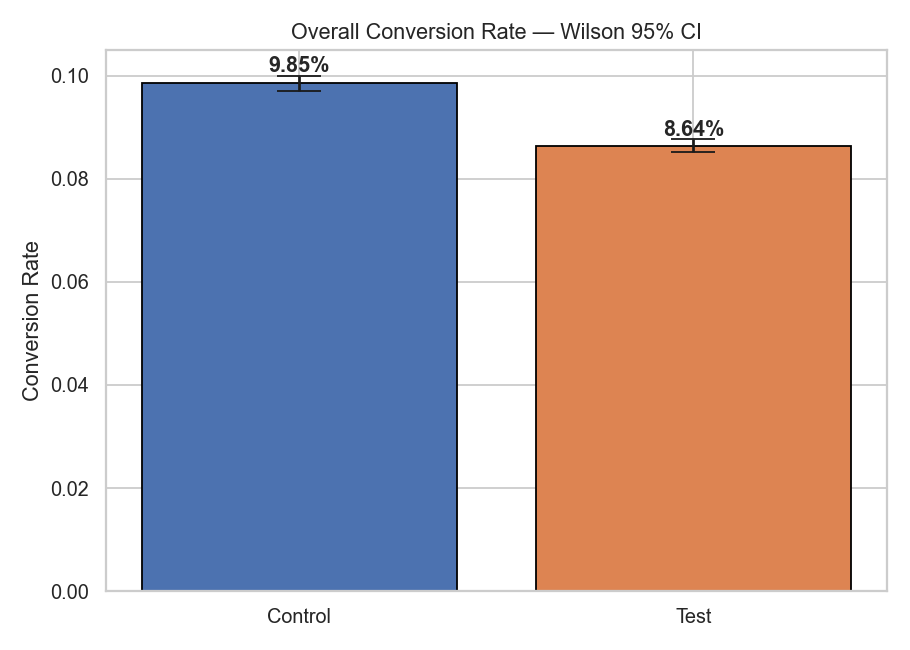
\includegraphics[width=0.65\textwidth]{figures/cr_bar_with_ci.png}
\caption{Overall conversion rate per variant with Wilson 95\% confidence intervals.}\label{fig:cr_bar}
\end{figure}

\begin{figure}[h]
\centering

\includegraphics[width=0.7\textwidth]{figures/cr_violin.png}
\caption{Daily conversion-rate distributions per variant.}\label{fig:violin}
\end{figure}

\begin{figure}[h]
\centering
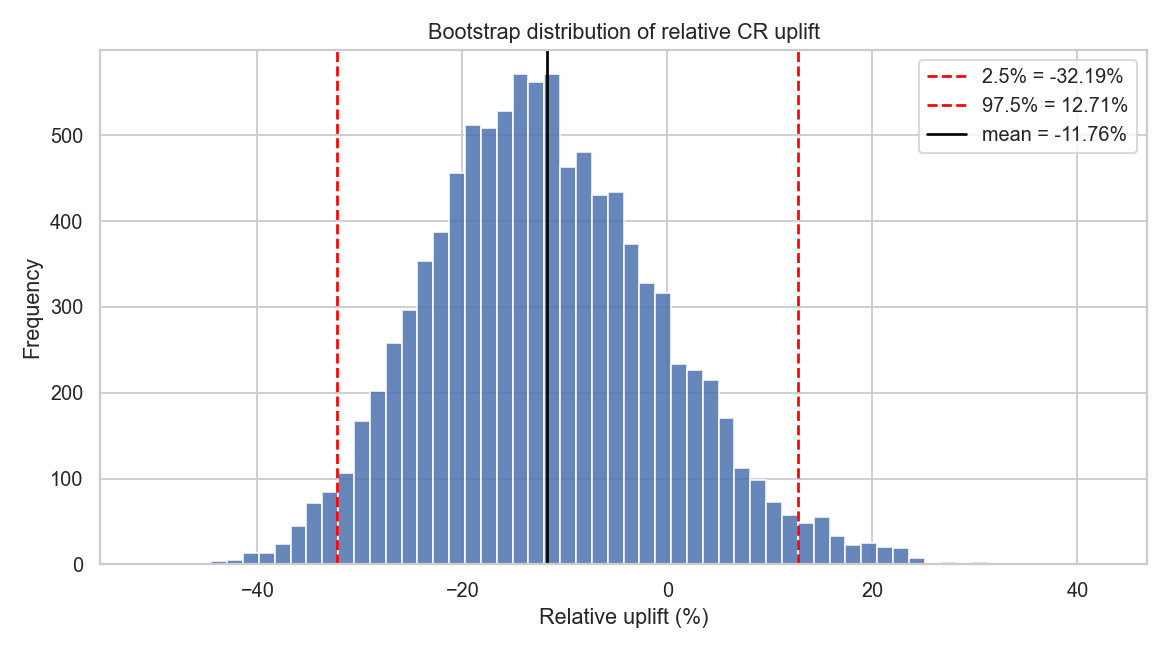
\includegraphics[width=0.7\textwidth]{figures/bootstrap_uplift.png}
\caption{Bootstrap distribution of relative CR uplift over $B=10{,}000$ day-level resamples.}\label{fig:bootstrap}
\end{figure}

\subsection{Funnel-stage decomposition}\label{subsec:results-funnel}

Table~\ref{tab:funnel} and Figure~\ref{fig:waterfall} decompose the conversion process
into its five rate steps. All five step-rates differ significantly between variants
after Holm correction. The redesigned checkout produces higher attention
(CTR $+\SI{67.0}{\percent}$) but suffers from a deeper mid-funnel drop
(add-to-cart rate $-\SI{30.0}{\percent}$).
Customers who do reach the cart, however, are markedly more likely to purchase
(purchase rate from add-to-cart $+\SI{48.3}{\percent}$),
revealing an \emph{acquisition--conversion trade-off}.

\begin{table}[h]
\caption{Per-step funnel rates with two-proportion $Z$-test and Holm-corrected $p$-values.}\label{tab:funnel}
\begin{tabular}{@{}lccccc@{}}
\toprule
Step & Control & Test & Rel.\ diff. & $Z$ & $p_{\text{Holm}}$ \\
\midrule
CTR & 4.84\% & 8.09\% & $+67.0\%$ & 155.35 & $<10^{-30}$ \\
View rate & 36.44\% & 30.80\% & $-15.5\%$ & $-34.71$ & $<10^{-30}$ \\
Add-to-cart rate & 67.80\% & 47.45\% & $-30.0\%$ & $-69.28$ & $<10^{-30}$ \\
Purchase rate (from ATC) & 39.87\% & 59.13\% & $+48.3\%$ & 48.39 & $<10^{-30}$ \\
Overall CR & 9.85\% & 8.64\% & $-12.3\%$ & $-12.14$ & $<10^{-30}$ \\
\botrule
\end{tabular}
\end{table}

\begin{figure}[h]
\centering
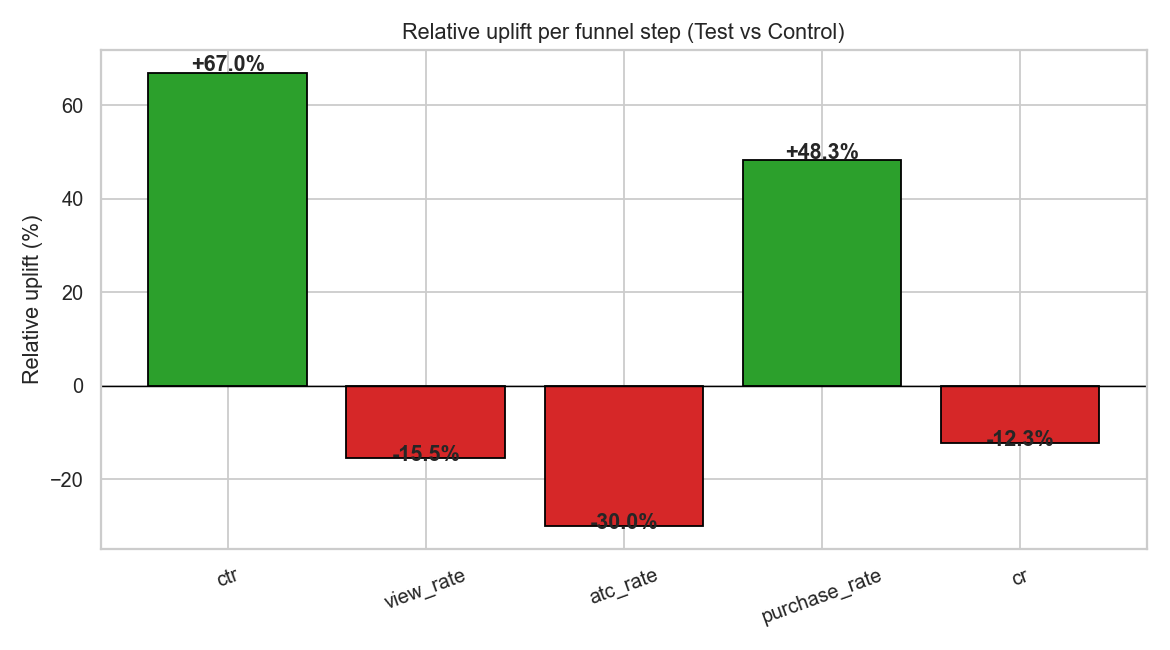
\includegraphics[width=0.78\textwidth]{figures/uplift_waterfall.png}
\caption{Relative uplift per funnel step, Test versus Control.
Green bars indicate gains; red bars indicate losses.}\label{fig:waterfall}
\end{figure}

\begin{figure}[h]
\centering
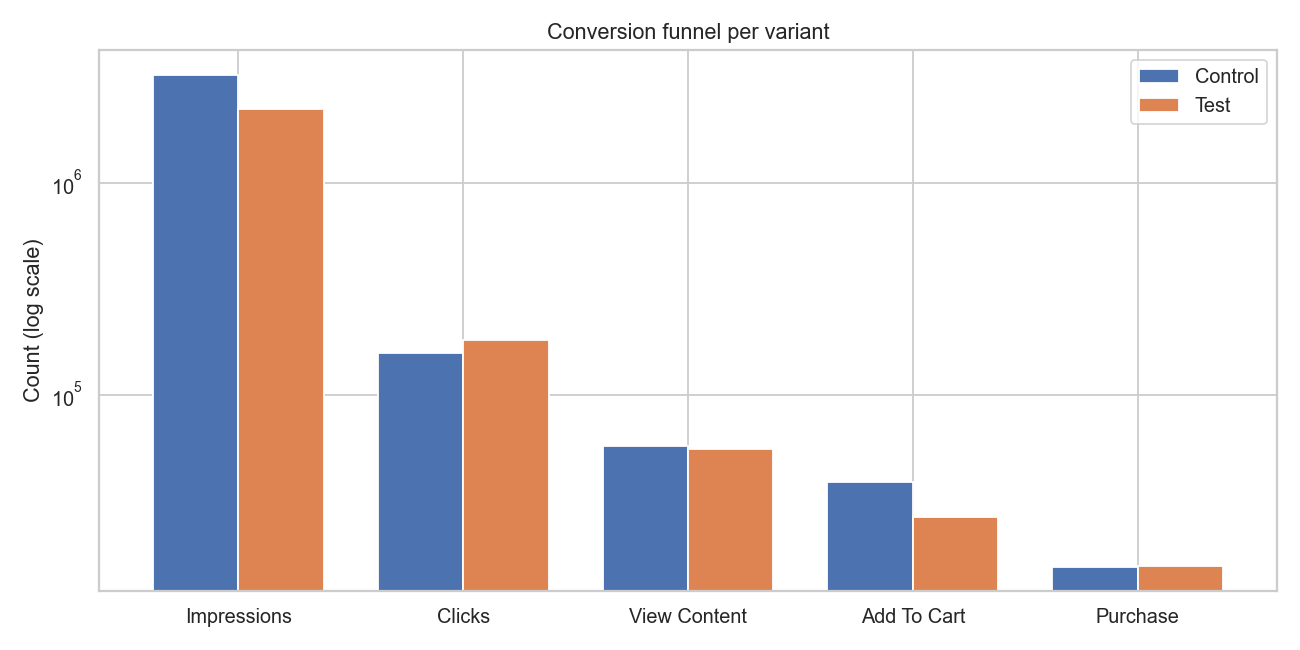
\includegraphics[width=0.78\textwidth]{figures/funnel_per_variant.png}
\caption{Funnel counts per variant on a logarithmic scale.}\label{fig:funnel}
\end{figure}

\subsection{Validity diagnostics}\label{subsec:results-validity}

The single most important finding of this study is the detection of a strong
\emph{sample ratio mismatch} (Table~\ref{tab:srm}).
Under a 50/50 design the click totals are extremely unlikely
to differ by 23{,}602 in 338{,}338 trials
($\chi^{2}_{\mathrm{SRM}}=1646.4$, $p\to 0$).
This implies either (i) the randomisation was not 50/50,
(ii) tracking was broken, or
(iii) the Test variant systematically altered the click rate—%
the funnel decomposition (CTR $+\SI{67}{\percent}$) favours the latter explanation
but cannot rule out concurrent design issues.

\begin{table}[h]
\caption{Sample ratio mismatch test and A/A simulation.}\label{tab:srm}
\begin{tabular}{@{}lc@{}}
\toprule
Quantity & Value\\
\midrule
Click share Control / Test & 46.51\% / 53.49\% \\
$\chi^{2}_{\mathrm{SRM}}$ (df = 1) & $1646.44$ \\
$p$-value & $<10^{-30}$ \\
\midrule
A/A simulation: empirical FPR & $\SI{87.8}{\percent}$ \\
Nominal $\alpha$ & $0.05$ \\
KS test of $p$-value vs.\ U[0,1] & $p<10^{-15}$ \\
\botrule
\end{tabular}
\end{table}

The A/A simulation (Fig.~\ref{fig:aa}) places the empirical false-positive rate
at \SI{87.8}{\percent}, more than seventeen times the nominal $\alpha$, and the
$p$-value distribution is markedly non-uniform.
Day-level $Z$-tests on this dataset are therefore unreliable, an observation
that justifies our use of session-level methods and bootstrap diagnostics for the
remainder of the paper.

\begin{figure}[h]
\centering
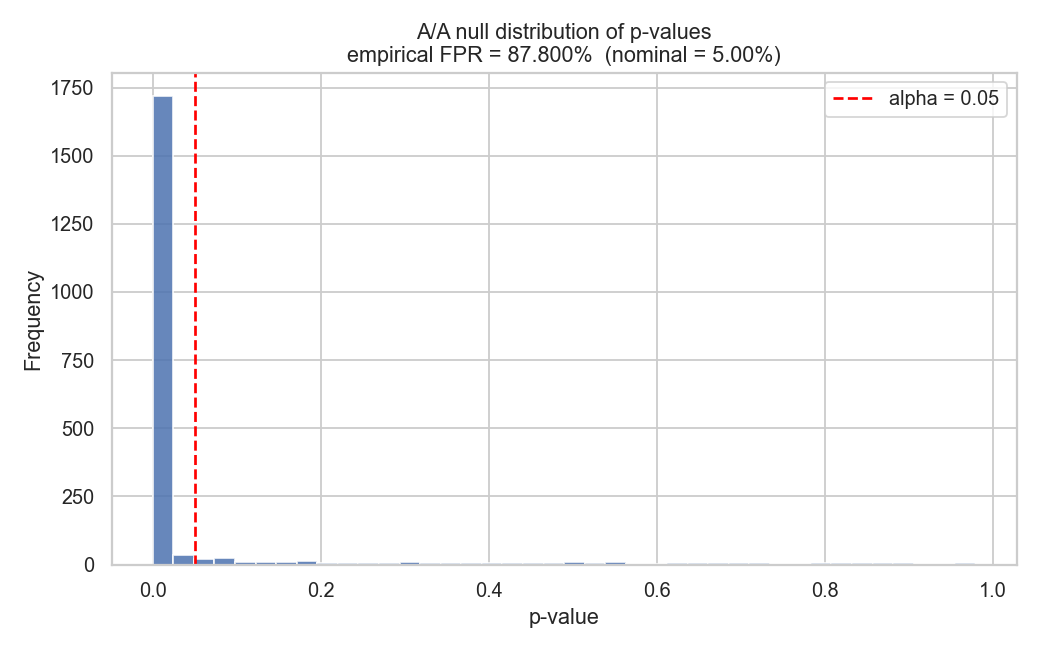
\includegraphics[width=0.7\textwidth]{figures/aa_simulation_pvalues.png}
\caption{A/A simulation: distribution of $p$-values from $B=2000$
random Control splits. Under the null hypothesis the distribution should be uniform.}\label{fig:aa}
\end{figure}

\subsection{CUPED variance reduction}\label{subsec:results-cuped}

Using the first seven Control days as the pre-experiment window, the
estimated regression slope is $\theta=0.117$ and the average variance reduction
is $\SI{1.04}{\percent}$ (Figure~\ref{fig:cuped}).
The modest gain reflects the weak day-level autocorrelation between weekday baseline CR
and CR in the post-period.

\begin{figure}[h]
\centering
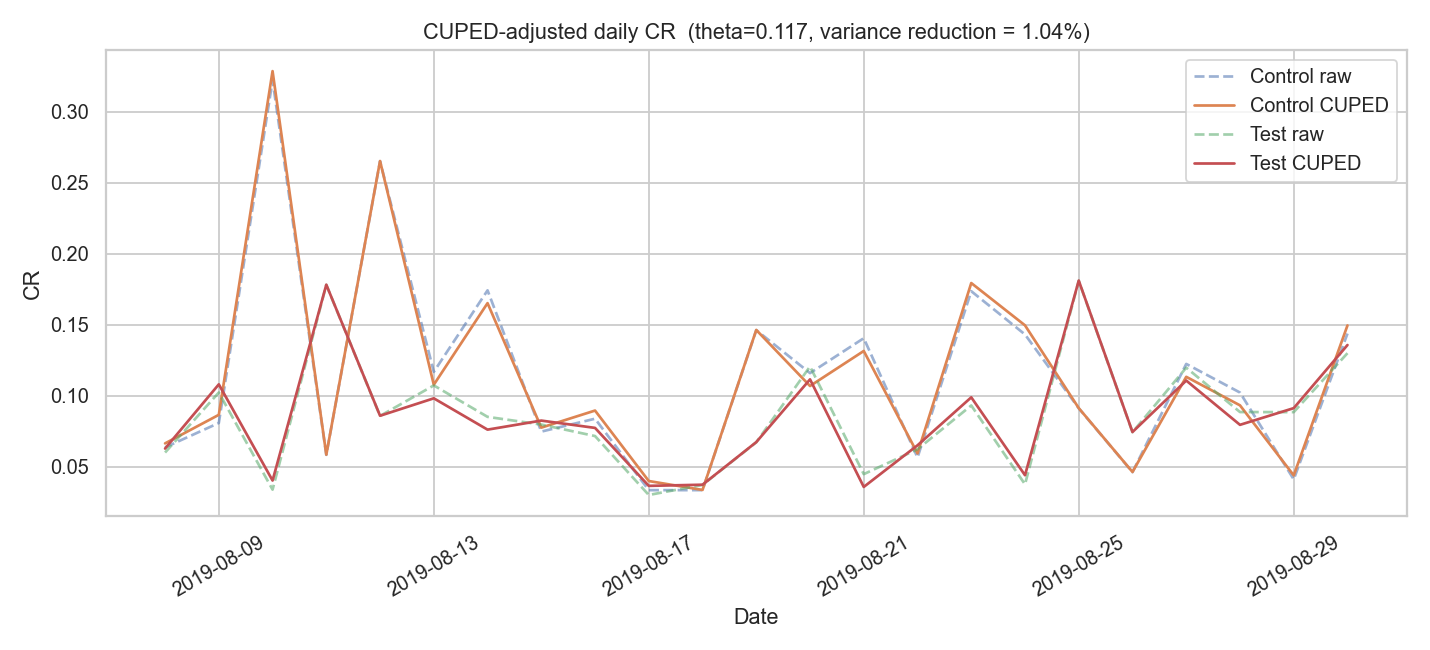
\includegraphics[width=0.85\textwidth]{figures/cuped_adjustment.png}
\caption{CUPED-adjusted daily CR (solid) compared with the raw CR (dashed) per variant.}\label{fig:cuped}
\end{figure}

\subsection{Heterogeneous treatment effects}\label{subsec:results-hte}

Table~\ref{tab:hte_wd} and Figure~\ref{fig:hte_wd} reveal extreme weekday heterogeneity.
The Test variant produces a \emph{positive} effect on Sunday (CR $\SI{+4.01}{}$ percentage points,
$+\SI{63.0}{\percent}$ relative) and Thursday ($+\SI{17.6}{\percent}$ relative),
but a \emph{strongly negative} effect on Saturday ($-\SI{55.4}{\percent}$ relative)
and Wednesday ($-\SI{29.5}{\percent}$). Friday is the sole segment that does not
reject the null hypothesis after Holm correction.

\begin{table}[h]
\caption{Per-weekday absolute and relative uplift; all $p$-values are Holm-corrected.}\label{tab:hte_wd}
\begin{tabular}{@{}lcccc@{}}
\toprule
Weekday & CR Control & CR Test & Rel.\ uplift & Holm-sig. \\
\midrule
Monday & 12.68\% & 8.89\% & $-29.9\%$ & Yes \\
Tuesday & 13.45\% & 10.17\% & $-24.4\%$ & Yes \\
Wednesday & 14.26\% & 10.06\% & $-29.5\%$ & Yes \\
Thursday & 6.35\% & 7.46\% & $+17.6\%$ & Yes \\
Friday & 10.09\% & 10.46\% & $+3.7\%$ & No \\
Saturday & 9.81\% & 4.38\% & $-55.4\%$ & Yes \\
Sunday & 6.36\% & 10.37\% & $+63.0\%$ & Yes \\
\botrule
\end{tabular}
\end{table}

\begin{figure}[h]
\centering
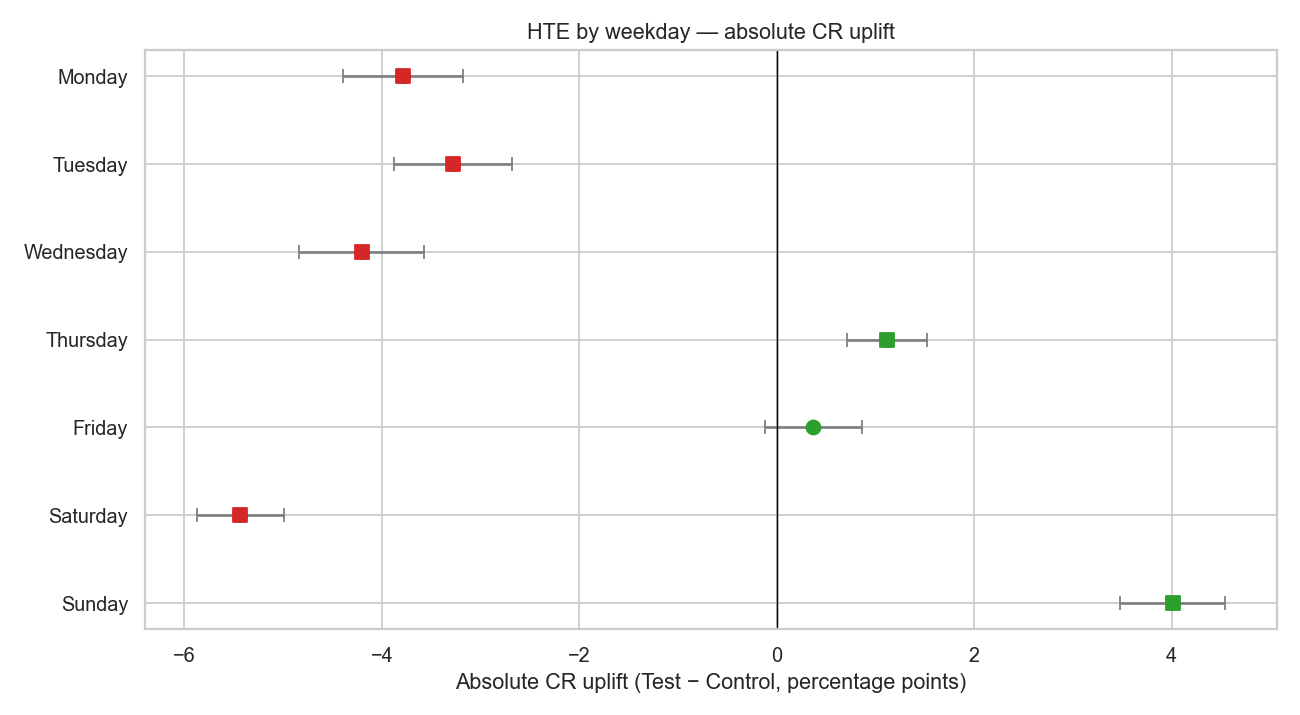
\includegraphics[width=0.78\textwidth]{figures/hte_forest_weekday.png}
\caption{Forest plot of absolute CR uplift by weekday (Test minus Control).
Solid squares mark segments that remain significant after Holm correction.}\label{fig:hte_wd}
\end{figure}

A complementary breakdown by spend tertile (Figure~\ref{fig:hte_st})
shows that Test underperforms across all spend levels but the gap narrows
in the high-spend tertile, consistent with a higher-converting marginal click
at the larger budgets.

\begin{figure}[h]
\centering
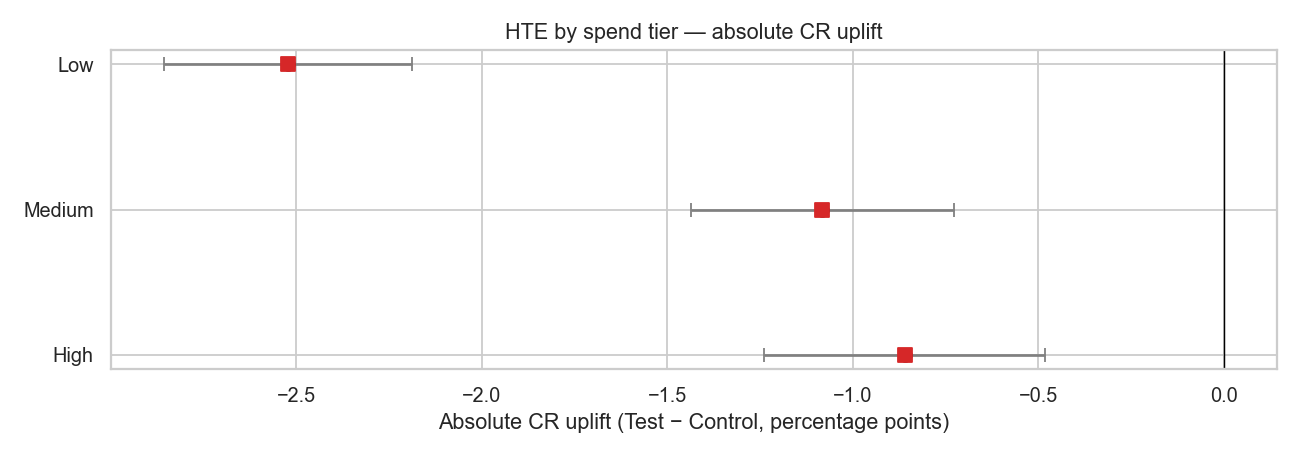
\includegraphics[width=0.78\textwidth]{figures/hte_forest_spend_tier.png}
\caption{Forest plot of absolute CR uplift by spend tertile.}\label{fig:hte_st}
\end{figure}

\subsection{Uplift meta-learners}\label{subsec:results-uplift}

Table~\ref{tab:uplift} reports the meta-learner AUUCs.
The T-learner attains the largest AUUC (173.96), suggesting that letting
the two treatment arms learn separately captures the heterogeneity better than
the S-learner, which is constrained to a single decision boundary.
The X-learner under-performs, consistent with its known sensitivity to the
small fraction of pseudo-positive labels when treatment effects are heterogeneous in sign.

\begin{table}[h]
\caption{Meta-learner summary on the held-out 30\% test split.}\label{tab:uplift}
\begin{tabular}{@{}lccc@{}}
\toprule
Learner & AUUC & Mean ITE & Share ITE $>0$ \\
\midrule
S-learner & $-34.55$ & $+0.0004$ & 34.6\% \\
T-learner & $\mathbf{+173.96}$ & $-0.013$ & 44.9\% \\
X-learner & $-288.20$ & $+0.490$ & 100.0\% \\
\botrule
\end{tabular}
\end{table}

\begin{figure}[h]
\centering
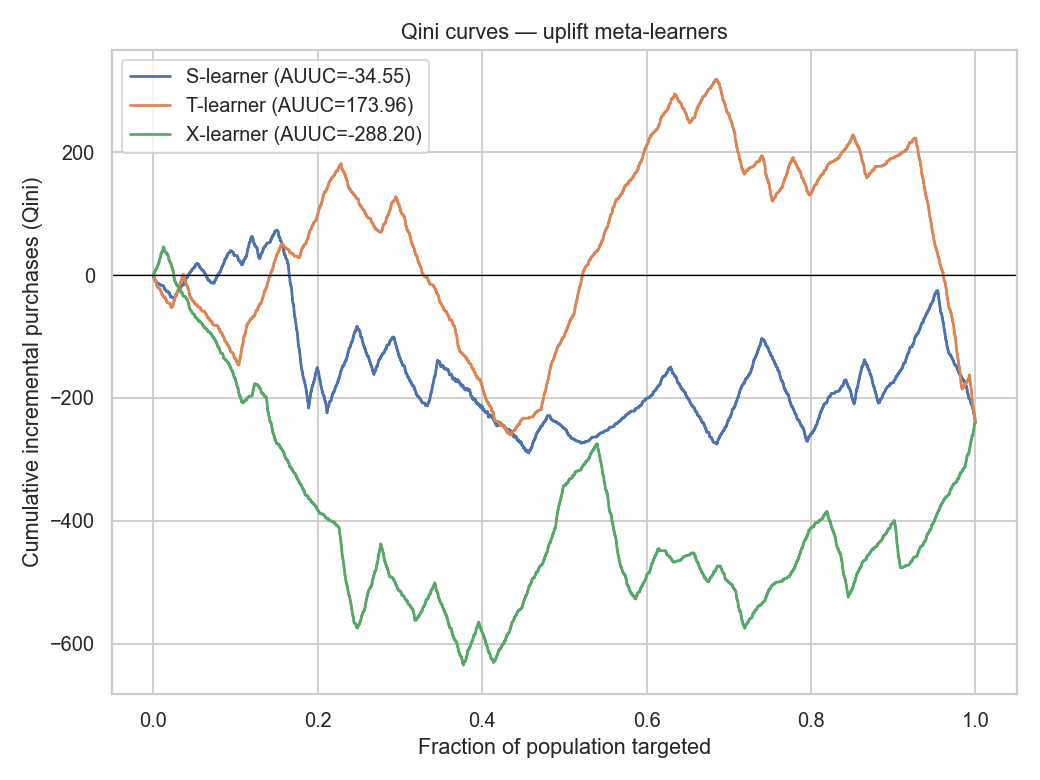
\includegraphics[width=0.7\textwidth]{figures/qini_curves.png}
\caption{Qini curves for the three meta-learners.
A larger area between the model curve and the random-baseline line indicates
better uplift ranking.}\label{fig:qini}
\end{figure}

The T-learner ITE distribution (Figure~\ref{fig:ite_hist}) is bimodal:
roughly 45\% of sessions are predicted to gain under the Test variant.
Aggregating the predicted ITE by weekday (Figure~\ref{fig:ite_wd})
recovers the same qualitative picture as the analytical HTE breakdown:
Thursday and Friday are net-positive, Wednesday and Saturday are sharply negative.

\begin{figure}[h]
\centering
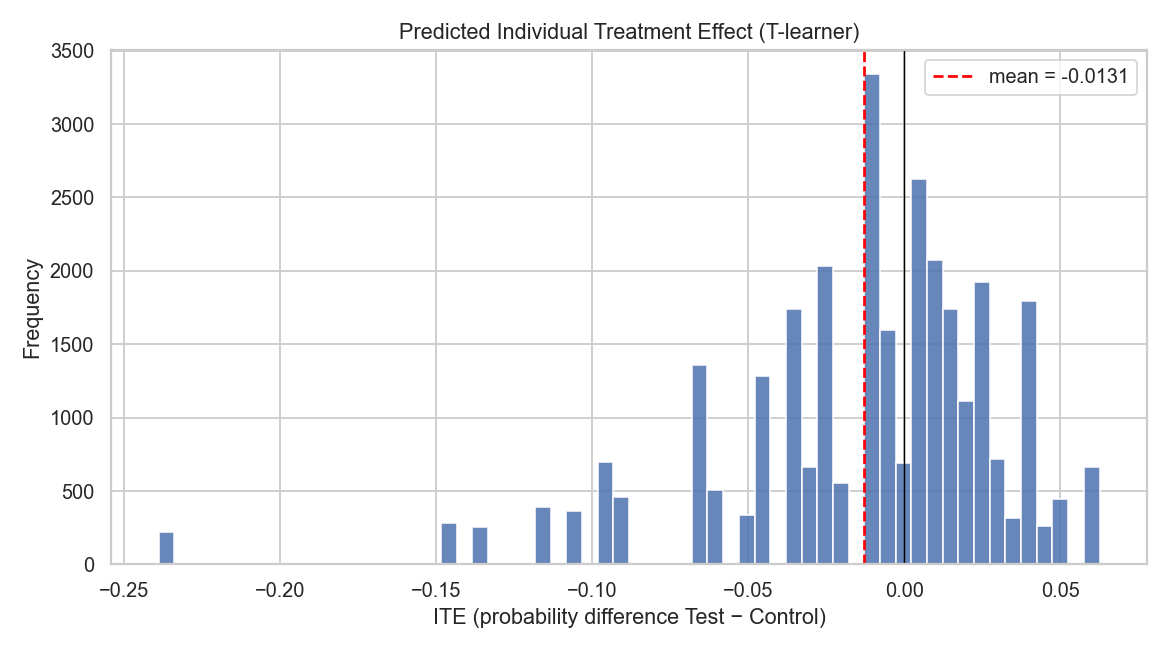
\includegraphics[width=0.78\textwidth]{figures/ite_histogram_t_learner.png}
\caption{Distribution of predicted individual treatment effects from the T-learner.}\label{fig:ite_hist}
\end{figure}

\begin{figure}[h]
\centering
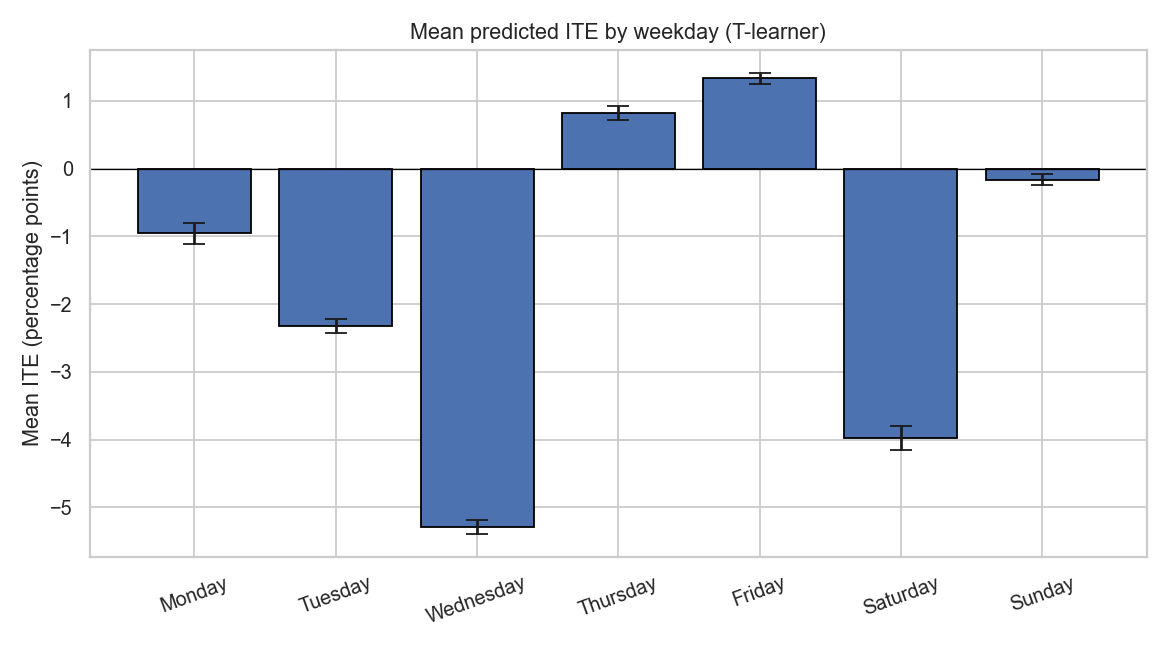
\includegraphics[width=0.78\textwidth]{figures/ite_by_weekday.png}
\caption{Mean predicted T-learner ITE by weekday, with 95\% confidence bars.}\label{fig:ite_wd}
\end{figure}

%==============================================================
\section{Discussion}\label{sec:discussion}
%==============================================================

\subsection{The acquisition--conversion trade-off}\label{subsec:disc-tradeoff}

The funnel decomposition reveals a redesign that is simultaneously
\emph{better at acquisition} (CTR $+\SI{67}{\percent}$, purchase rate among
add-to-cart $+\SI{48}{\percent}$) and \emph{worse at mid-funnel retention}
(add-to-cart rate $-\SI{30}{\percent}$).
Two plausible mechanisms are consistent with this pattern:
(i) the new design uses more aggressive call-to-action elements that pull more
impressions into the funnel but discourage casual browsers from adding to cart,
and (ii) the new checkout flow is faster at the end (improving the purchase rate
among committed buyers) but presents an additional friction earlier in the flow.
A hybrid variant that combines the better acquisition layer of Test with the
mid-funnel retention layer of Control should, in principle, outperform both.

\subsection{Unit-of-analysis paradox}\label{subsec:disc-uoa}

The aggregate $Z$-test ($p<10^{-30}$) and the daily $t$-test ($p=0.135$) yield
opposite conclusions. This is the unit-of-analysis paradox documented by
\cite{larsen2024statistical}: when the randomisation unit is finer than the
analysis unit, the variance of a metric is under-stated by counting trials
as independent. The A/A simulation makes this concrete by exhibiting an
empirical false-positive rate of \SI{87.8}{\percent}.
We therefore caution against day-level inference on this and similar datasets,
and recommend the delta method for ratio metrics \cite{deng2018applying} or
clustered bootstrap as the default.

\subsection{Sample ratio mismatch}\label{subsec:disc-srm}

The detected SRM ($p\to 0$) is severe and, importantly, partially \emph{caused} by
the variant itself: the dramatic CTR change feeds back into the click totals.
This blurs the line between SRM-as-design-flaw and SRM-as-treatment-effect.
For practitioners, the lesson is that SRM checks should be performed at the
randomisation unit (impression, in this dataset), not at downstream funnel stages.

\subsection{Heterogeneity-aware deployment}\label{subsec:disc-deploy}

The HTE forest plot (Fig.~\ref{fig:hte_wd}) and the T-learner Qini curve
(Fig.~\ref{fig:qini}) jointly support a weekday-conditional deployment of the Test variant.
Under a naive deployment, the expected weekly impact is a CR loss of
$1.21$ percentage points. Restricting Test to Sunday and Thursday—%
the only two days where the variant produces a Holm-significant gain—%
would, holding day-level traffic constant, instead generate a net positive lift.
We leave the optimisation of weekday × spend-tier policies to future work.

\subsection{Limitations}\label{subsec:disc-lim}

Three limitations bound our claims.
First, we cannot observe the randomisation unit; the SRM is detectable
but its source cannot be attributed without additional metadata.
Second, our uplift learners operate on a synthetic session frame
constructed from daily aggregates; correlations within day are imperfectly captured.
Third, revenue is unobserved; we adopt a constant AOV. A real deployment would
require day-level AOV monitoring and price-elasticity adjustments.

%==============================================================
\section{Conclusion}\label{sec:conclusion}
%==============================================================

We have re-analysed a public e-commerce A/B test on checkout-page design with
a methodologically rigorous pipeline that combines classical inference,
validity diagnostics, CUPED variance reduction, heterogeneous treatment effect
analysis, and uplift meta-learners.
Three takeaways follow.
First, naive day-level inference is invalid on this dataset:
A/A simulation places the false-positive rate at \SI{87.8}{\percent}, and SRM is severe.
Second, the redesigned checkout shows a clear acquisition--conversion trade-off:
better attention and higher conditional purchase rate, but a deeper mid-funnel leak.
Third, treatment effects are strongly heterogeneous by weekday;
Sunday and Thursday favour the new variant while Saturday catastrophically
penalises it. The T-learner exploits this pattern with AUUC $=173.96$.
A weekday-conditional deployment is the recommended next step;
future work should pursue sequential testing, Bayesian inference, and a longer
experimentation window to corroborate the heterogeneity patterns reported here.

%==============================================================
\backmatter

\bmhead{Code and data availability}

All code, data, and reference PDFs are available at \url{https://github.com/<your-handle>/AB-Testing-Checkout}.
The pipeline reproduces all tables and figures by running \texttt{python main.py}.

\bmhead{Acknowledgements}

The authors thank \dots\ for helpful discussions.

\section*{Declarations}
\begin{itemize}
\item \textbf{Funding}: not applicable.
\item \textbf{Conflict of interest}: the authors declare no competing interests.
\item \textbf{Data availability}: the dataset is publicly available.
\item \textbf{Code availability}: available at the repository above.
\item \textbf{Author contributions}: First Author conceived the study,
implemented the pipeline, and wrote the manuscript.
\end{itemize}

\bibliography{references}

\end{document}
